%!TEX root = ../DA_MainDocument.tex
\chapter{Theoretische Grundlagen}

\section{Mobile Reiseorganisation und digitale Workflows}
\subsection{Charakteristika von Reisedaten und deren Verwaltung}
Reisedaten umfassen Fluginformationen, Buchungsdaten, Dokumente, Belege und Erinnerungen. Diese Informationen werden in der Praxis häufig in unterschiedlichen Medien und Systemen gespeichert (E-Mail, Dateien, Kalender, Papier), was zu Fragmentierung führt.

\subsection{Herausforderungen bei der Fragmentierung von Reiseinformationen}
Die Verteilung erschwert die strukturierte Organisation, verlängert Suchvorgänge und reduziert die Nachvollziehbarkeit im Unternehmenskontext. Ohne strukturierte Ablage entstehen organisatorische Fehler und ein hoher manueller Aufwand.

\section{Grundlagen des automatischen Imports}
\subsection{Zielsetzung und Nutzen}
Automatisierter Import reduziert manuellen Aufwand und senkt die Fehlerquote. Ziel ist es, Flugdaten möglichst schnell und korrekt zu erfassen, um den Nutzer von repetitiven Eingaben zu entlasten und die Datenqualität zu erhöhen.

\subsection{Abgrenzung zu manueller Erfassung}
Manueller Import bleibt als Fallback bestehen, ist aber zeitaufwändiger und fehleranfälliger. Automatisierung steigert Komfort und Konsistenz.

\subsection{Typische Fehlerquellen bei Importen}
Typische Probleme sind unvollständige Daten, fehlerhafte OCR-Erkennung oder unklare Codierung in QR/BCBP. Daher sind Validierung und Nachbearbeitung wichtig.

\subsection{Datenquellen für Flugdaten}
\subsubsection{QR-Code / Boarding Pass (BCBP)}
Boardingpässe enthalten standardisierte BCBP-Daten, die sich strukturiert auslesen lassen \cite{iataBCBP}. BCBP basiert auf festen Positionsfeldern. Die Struktur ermöglicht die Extraktion von Airline, Flugnummer, Datum und Airports \cite{iataBCBP}. Kernfelder sind Abflug-/Zielairport, Flugnummer und Datum. Diese reichen für einen validen Flight-Import aus. Nicht alle Boardingpässe sind standardkonform; zudem fehlen häufig Zusatzdaten wie Gate oder Sitzplatz.

\subsubsection{OCR aus Bildern/Dokumenten}
OCR ermöglicht Import aus Fotos und PDFs, wenn kein QR-Code vorhanden ist. Schriftgröße, Kontrast und Bildrauschen beeinflussen die Genauigkeit der OCR. Nach OCR müssen Texte geparst und relevanten Feldern zugeordnet werden. Fehlerhafte OCR wird durch Plausibilitätschecks abgefangen, z.\,B. IATA-Codes oder Datumsformate.

\subsubsection{E-Mail-Import (Buchungsdaten)}
Buchungsbestätigungen enthalten strukturierte Informationen, die per Parser ausgelesen werden können. Typische Mails enthalten Buchungsreferenz, Routing, Zeiten und Passagierdaten. Format und Layout unterscheiden sich je Airline. Unterschiedliche Templates erfordern flexible Parser oder heuristische Regeln.

\subsection{Technische Anforderungen}
Der Import muss technisch stabil, verifizierbar und nutzerfreundlich sein. Validierung prüft Plausibilität (Datum, Airport-Codes). Feld-Mapping normalisiert externe Daten. Deduplizierung erkennt Mehrfachimporte. Fallback-Strategien und manuelle Ergänzung bei unvollständigen Daten sind erforderlich. Asynchrone Verarbeitung hält die UI responsiv. Fehler müssen nutzerfreundlich kommuniziert werden.

\subsection{Vergleich: Manuell vs.\ Automatisch}
Automatisierung reduziert Zeitaufwand und Fehlerquote, steigert Nutzerakzeptanz, Wiederholbarkeit und Skalierbarkeit.

\section{Grundlagen visueller Flugrouten-Darstellung}
\subsection{Charakteristika und Nutzen}
Die visuelle Darstellung von Flugrouten dient der Orientierung und der schnellen Übersicht über Reisehistorie und geplante Flüge. Routen sollen geografisch korrekt auf einer Karte dargestellt und mit Interaktion verbunden sein.

\subsection{Anforderungen an eine mobile Flugrouten-Karte}
Die Karte muss auf mobilen Geräten performant laufen, interaktiv bedienbar sein und darf die Nutzerführung nicht überladen. Performance \& Ladezeiten, Skalierbarkeit bei vielen Flügen, mobile Optimierung (Touch, Displaygrößen), Genauigkeit der Darstellung (geodätisch korrekt, nicht als gerade Linie) und Usability (Fokus, Zoom, Auswahl) \cite{reactNativeMaps,movableTypeLatLong}.

\subsection{Technische Grundlagen der Routenberechnung}
Die Routen werden anhand geographischer Koordinaten der Airports berechnet. Für die Distanz zwischen zwei Airports wird die Haversine-Formel verwendet \cite{movableTypeLatLong}. Die Flugroute wird als Great-Circle-Bogen modelliert. Flugfortschritt in Echtzeit wird über departureAt/arrivalAt interpoliert.

\section{Proaktive Benachrichtigungssysteme und Erinnerungsmanagement}

Proaktive Benachrichtigungssysteme verfolgen das Ziel, relevante Informationen nicht erst auf explizite Nutzeranfrage bereitzustellen, sondern situations- und zeitgerecht automatisch auszuliefern. In der Literatur wird diese Logik häufig als Gegenüberstellung von \glqq Push\grqq{} (System initiiert die Informationsbereitstellung) und \glqq Pull\grqq{} (Nutzer initiiert die Informationsabfrage) diskutiert \cite{mehrotra2018intelligent}. Push-Ansätze sind insbesondere dann sinnvoll, wenn Handlungen an Zeitfenster gebunden sind oder wenn das Versäumen einer Handlung hohe Kosten verursacht (z.\,B. verpasster Check-in oder Gate-Schluss).

Reiseorganisation ist ein prototypischer Anwendungsfall für proaktive Erinnerungssysteme, weil zentrale Prozessschritte (Online-Check-in, Gepäckaufgabe, Sicherheitskontrolle, Boarding) in der Praxis durch harte oder \glqq quasi-harte\grqq{} Deadlines strukturiert sind \cite{britishAirwaysCheckin,lufthansaCheckin,austrianCheckin,viennaAirportOnlineCheckin,klmBoarding}. Die praktische Relevanz zeigt sich auch daran, dass die Reiseindustrie bereits proaktive Muster etabliert hat: Beispielsweise der automatische Versand von Bordkarten an Reisende. Solche Mechanismen externalisieren Erinnerungsarbeit und sind damit eine Blaupause für digitale Reiseassistenten wie Skyline.

Gleichzeitig ist Reiseorganisation kognitiv anspruchsvoll, weil sie mehrere parallele Zukunftsintentionen umfasst (Dokumente prüfen, Abfahrtszeit planen, Gate wechseln, Belege sichern) und weil sich Parameter dynamisch ändern können. In dieser Dynamik entsteht ein Spannungsfeld: Benachrichtigungen sollen rechtzeitig und hilfreich sein, dürfen aber nicht zur Überlastung beitragen (Notification Fatigue) oder in unpassenden Momenten stören \cite{pielot2014notifications,mehrotra2016myphone}.

\subsection{Proaktivität und Push/Pull in Benachrichtigungssystemen}

In der HCI- und Informatikforschung wird \glqq proaktiv\grqq{} nicht nur als \glqq früh\grqq{} verstanden, sondern als Eigenschaft eines Systems, \textbf{auf eigene Initiative} und \textbf{im Sinne des Nutzers} zu handeln \cite{tennenhouse2000proactive,coronado2010continuous}. Reaktive Systeme liefern Informationen primär dann, wenn eine Nutzerinteraktion dies auslöst (Suche, Klick, Öffnen einer App). Proaktive Systeme verschieben die Verantwortung für Timing und Erinnern teilweise zurück zum System: Sie erkennen günstige Zeitpunkte, liefern Hinweise und reduzieren damit typische Fehlerklassen wie \glqq zu spät bemerkt\grqq{} oder \glqq vergessen\grqq{} \cite{mehrotra2018intelligent}. Diese Entlastungslogik ist eng verwandt mit dem Konzept des kognitiven Offloadings.

\begin{figure}[htbp]
  \centering
  \includegraphics[width=0.15\textwidth]{notification_icon}
  \caption{Symbol für Benachrichtigungen (Push-Trigger). Quelle: \cite{wikimediaNotificationIcon}}
  \label{fig:notification_icon}
\end{figure}

Die Push/Pull-Unterscheidung ist eine Frage der Nutzerintention und Disruption: Push-Systeme können hohe Nützlichkeit erzielen, erzeugen aber das Risiko, Aufmerksamkeit in unpassenden Situationen zu beanspruchen; Pull-Systeme minimieren Disruption, bergen aber das Risiko, dass kritische Informationen nicht rechtzeitig abgerufen werden \cite{mehrotra2018intelligent}. Für Skyline folgt daraus eine zentrale Designhypothese: Proaktivität ist dann gerechtfertigt, wenn das System (a) einen stabilen Anlass hat (z.\,B. Abflugzeit), (b) eine konkrete Handlung ermöglicht (z.\,B. Check-in öffnen) und (c) das Risiko von Störung durch Quiet Hours und Nutzerkontrolle begrenzt \cite{androidNotifications,applePushPrimer2020}.

\begin{figure}[htbp]
  \centering
  \includegraphics[width=0.7\textwidth]{push_subscribe}
  \caption{Publish/Subscribe-Schema (Push-Prinzip): Der Server liefert Informationen proaktiv an den Client. Quelle: \cite{wikimediaPushSubscribe}}
  \label{fig:push_subscribe}
\end{figure}

\begin{figure}[htbp]
  \centering
  \includegraphics[width=0.6\textwidth]{polling_pull}
  \caption{Polling-System (Pull-Prinzip): Der Client fragt periodisch beim Server ab. Quelle: \cite{wikimediaPolling}}
  \label{fig:polling_pull}
\end{figure}

\subsection{Kognitive Grundlagen der Erinnerungslast}

Reisebezogene Aufgaben lassen sich als Fälle des \textbf{prospektiven Gedächtnisses} (Prospective Memory) modellieren: das Erinnern, eine beabsichtigte Handlung in der Zukunft auszuführen, häufig ausgelöst durch Zeitpunkte oder Ereignisse \cite{jones2021prospectivememory,ball2024reminders}. Prospective-Memory-Aufgaben sind in der Reiseorganisation besonders fehleranfällig, weil sie mit konkurrierenden Anforderungen interferieren. Ein zentraler Befund ist, dass Menschen externe Hilfen (Notizen, Kalender, Reminder) nutzen, um die Kosten interner Kontrolle zu senken \cite{gilbert2023intentionoffloading}.

Das Konzept \textbf{Intention Offloading} beschreibt die Strategie, Absichten in externe Speicher zu verlagern. Für das Design von Skyline ist wichtig: Erinnerungen wirken zuverlässiger, wenn sie handlungsnah und handlungsfähig sind (z.\,B. \glqq jetzt einchecken\grqq{}), statt nur abstrakt zu informieren \cite{gilbert2023intentionoffloading,jones2021prospectivememory}.

\subsection{Notification Fatigue und Governance}

Unter \textbf{Notification Fatigue} wird verstanden, dass zu häufige oder als irrelevant erlebte Hinweise zu Abwertung, Ignorieren oder Deaktivieren führen \cite{pielot2014notifications,sahami2014largescale,mehrotra2016myphone}. Mobile-HCI-Feldstudien zeigen, dass Benachrichtigungen zwar nützlich sein können, aber oft als störend wahrgenommen werden, wenn Timing und Relevanz nicht zur aktuellen Situation passen \cite{mehrotra2016myphone}. Studien zur mobilen Receptivity belegen, dass \glqq richtig getimed\grqq{} oft wichtiger ist als \glqq mehr Informationen\grqq{} \cite{fischer2011investigating}.

Aus Governance-Sicht lassen sich drei Gestaltungsprinzipien ableiten: (1) \textbf{Relevanz vor Vollständigkeit}---Systeme sollten das melden, was eine konkrete Handlung ermöglicht \cite{androidNotifications}. (2) \textbf{Nutzerkontrolle und Transparenz}---Benachrichtigungen benötigen bewusste Zustimmung; Best Practices empfehlen, diese \textbf{im Kontext der Funktionalität} einzuholen \cite{applePushPrimer2020}. (3) \textbf{Schutzzeiten}---Quiet Hours bzw. Fokus-Modi begrenzen Störungen \cite{androidNotifications}.

\begin{figure}[htbp]
  \centering
  \includegraphics[width=0.5\textwidth]{android_notifications}
  \caption{Beispielhafte Notification-Interaktion in einer mobilen App (Nutzerkontrolle, Prioritäten). Quelle: \cite{wikimediaAndroidNotifications}}
  \label{fig:android_notifications}
\end{figure}

\subsection{Anforderungen und Heuristiken im Reise-Kontext}

Im Reise-Kontext variieren operative Fenster je Airline und Flughafen. Check-in-Fenster reichen von \glqq ca. 30 Stunden vor Abflug\grqq{} bis \glqq bis zu 30 Tage\grqq{}; Boarding beginnt typischerweise 60 bis 25 Minuten vor Abflug \cite{klmBoarding,britishAirwaysCheckin,lufthansaCheckin}. Flughäfen empfehlen Ankunftszeiten (z.\,B. 2--3 Stunden vor Abflug für internationale Flüge). Für Skyline werden daher \textbf{zeitbasierte Heuristiken} als Default-Regeln verwendet:

\begin{table}[htbp]
  \centering
  \caption{Zeitbasierte Heuristiken für Reise-Reminder (Skyline-relevant)}
  \label{tab:reminder_heuristiken}
  \begin{tabular}{lll}
    \textbf{Anlass} & \textbf{Trigger} & \textbf{Begründung} \\
    \midrule
    Check-in & T$-$24\,h & breit kompatibel, viele Check-in-Fenster $\geq$24\,h \\
    Dokumente & T$-$12\,h & Vorlauf für Pass/ID/Visa-Check \\
    Zum Flughafen & T$-$3\,h / T$-$2\,h & Lang-/Kurzstrecke, Flughafenempfehlungen \\
    Boarding & T$-$60\,min, T$-$30\,min & deckt Boardingspannen ab \\
    Belege/Quittungen & T+2\,h nach Ankunft & handlungsnah nach Reiseende \\
  \end{tabular}
\end{table}

Für dynamische Ereignisse (Verspätungen, Gate-Wechsel) reichen statische Heuristiken nicht aus. Abbildung~\ref{fig:departure_board} illustriert, wie Flughäfen Echtzeit-Informationen anzeigen; solche Daten werden typischerweise über kommerzielle APIs bereitgestellt \cite{flightawareAeroAPI,ciriumFlexAPIs,aviationstack}. Skyline nutzt die in der App gespeicherten \texttt{departureAt}/\texttt{arrivalAt}-Zeiten als Basis; Echtzeit-Updates würden zusätzliche API-Anbindungen erfordern.

\begin{figure}[htbp]
  \centering
  \includegraphics[width=0.7\textwidth]{departure_board}
  \caption{Abflugtafel als Beispiel für Echtzeit-Fluginformationen (Verspätungen, Gate). Quelle: \cite{wikimediaDepartureBoard}}
  \label{fig:departure_board}
\end{figure}

\subsection{Konzeption und technische Umsetzung (Skyline-relevant)}

Konzeptionell lässt sich ein proaktives Reise-Benachrichtigungssystem als Pipeline modellieren: (1) \textbf{Faktenbasis} (Flugobjekt mit departureAt/arrivalAt), (2) \textbf{Regelwerk} (Offsets/Heuristiken), (3) \textbf{Scheduler} (lokal und/oder serverseitig), (4) \textbf{Delivery} (Benachrichtigung + Deep Link), (5) \textbf{Kontrollschicht} (Quiet Hours, Opt-out). Skyline implementiert dies mit Expo Notifications \cite{expoNotifications}.

Triggerzeiten werden als Offsets relativ zu departureAt/arrivalAt berechnet. Technisch kritisch ist die Zeitzonen- und Sommerzeitkorrektheit. Für Persistenz sind hybride Strategien robust: lokale Persistenz ermöglicht Offline-Fähigkeit; serverseitige Persistenz ermöglicht Rescheduling bei Datenänderungen. Deep Links transformieren Benachrichtigungen von \glqq Info\grqq{} zu \glqq Handlung\grqq{}: Der Tap führt direkt in die Flugdetails \cite{applePushPrimer2020}. Das Berechtigungs-Prompt sollte nicht sofort, sondern \textbf{im Kontext der Funktion} (z.\,B. nach Anlegen eines Flugs) erscheinen \cite{applePushPrimer2020}. Fehlende oder ungültige Zeitpunkte werden abgefangen; bei widersprüchlichen Daten ist eine degradierte Strategie sinnvoll (nur statische Reminder oder Umstellung auf Pull).

\section{Zentrale Datenverwaltung und Sicherheit für eine mobile Reiseorganisations-App}

\subsection{Einordnung und Zielsetzung}
Eine mobile Reiseorganisations-App ist nur dann nachhaltig nützlich, wenn sie
(a) alle relevanten Reiseinformationen konsistent bündelt, (b) im Alltag schnell
Auskunft geben kann (\glqq Wann ist mein Boarding?\grqq{}, \glqq Wo ist mein Ticket?\grqq{})
und (c) trotz sensibler Datenlage ein belastbares Sicherheits- und
Datenschutzniveau erreicht. Diese Ziele sind direkt miteinander gekoppelt:
Verteilte Speicherung in E-Mails, Notizen, Screenshots und mehreren Apps erzeugt
Inkonsistenz, Suchaufwand und unkontrollierte Replikation sensibler Daten.

Im Geschäftsreise-Kontext kommt zusätzlich Nachweisbarkeit hinzu:
Buchungsinformationen, Belege und Änderungen müssen auditierbar und einem
konkreten Trip zuordenbar sein. Daraus folgt für die Architektur die
Grundentscheidung für eine zentrale, strukturierte Datenbasis (\textit{Single
Source of Truth}), kombiniert mit Datenintegrität, klarer Rechteverwaltung und
nachvollziehbarer Historie.

\begin{figure}[htbp]
  \centering
  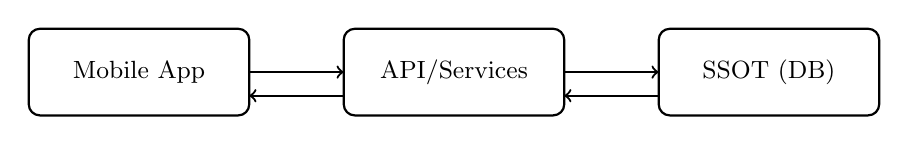
\begin{tikzpicture}[x=1cm,y=1cm]
    \draw[rounded corners, thick] (0,0) rectangle (2.8,1.1);
    \node at (1.4,0.55) {\small Mobile App};
    \draw[rounded corners, thick] (4,0) rectangle (6.8,1.1);
    \node at (5.4,0.55) {\small API/Services};
    \draw[rounded corners, thick] (8,0) rectangle (10.8,1.1);
    \node at (9.4,0.55) {\small SSOT (DB)};
    \draw[->, thick] (2.8,0.55) -- (4,0.55);
    \draw[->, thick] (6.8,0.55) -- (8,0.55);
    \draw[->, thick] (8,0.25) -- (6.8,0.25);
    \draw[->, thick] (4,0.25) -- (2.8,0.25);
  \end{tikzpicture}
  \caption{Zentraler Datenfluss mit einer kanonischen Datenquelle (SSOT).}
  \label{fig:ssot_dataflow}
\end{figure}

\subsection{Single Source of Truth und Datenkonsistenz}
SSOT beschreibt das Prinzip, dass jedes relevante Datenelement genau eine
massgebliche Pflege- und Referenzstelle besitzt. In der Reiseorganisation ist der
Nutzen besonders hoch, weil Daten typischerweise fragmentiert vorliegen
(Buchungsdaten in E-Mails, Dokumente als Fotos, Erinnerungen in Kalendern,
Notizen in separaten Apps). Eine zentrale Datenbasis reduziert doppelte Erfassung,
Inkonsistenzen und Update-Anomalien.

Konsistenz muss dabei in zwei Schichten betrachtet werden:
\begin{itemize}
  \item \textbf{Konsistenz in der Datenbank:} Schema, Constraints und
  Transaktionen erzwingen strukturell gültige Zustände
  \cite{postgresqlConstraints,postgresqlTxIsolation}.
  \item \textbf{Konsistenz über Geräte:} Offline-Phasen und parallele Zugriffe
  erzeugen Replikations- und Konfliktfragen; hier sind konsistente
  Synchronisationsregeln erforderlich \cite{capBrewer2012,dynamo2007}.
\end{itemize}

Die Normalisierung des Datenmodells ist dafür eine zentrale Grundlage, weil sie
Redundanz senkt und Änderungen an einer kanonischen Stelle bündelt.
\begin{figure}[htbp]
  \centering
  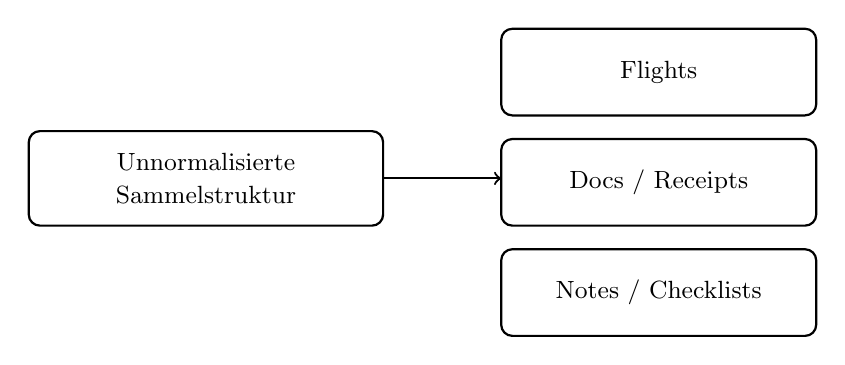
\begin{tikzpicture}[x=1cm,y=1cm]
    \draw[rounded corners, thick] (0,0) rectangle (4.5,1.2);
    \node[align=center] at (2.25,0.6) {\small Unnormalisierte\\\small Sammelstruktur};
    \draw[->, thick] (4.5,0.6) -- (6,0.6);
    \draw[rounded corners, thick] (6,1.4) rectangle (10,2.5);
    \node[align=center] at (8,1.95) {\small Flights};
    \draw[rounded corners, thick] (6,0) rectangle (10,1.1);
    \node[align=center] at (8,0.55) {\small Docs / Receipts};
    \draw[rounded corners, thick] (6,-1.4) rectangle (10,-0.3);
    \node[align=center] at (8,-0.85) {\small Notes / Checklists};
  \end{tikzpicture}
  \caption{Konzeptuelle Normalisierung: von Sammeldaten zu klaren Entitäten.}
  \label{fig:normalization_concept}
\end{figure}

Für die Synchronisation zwischen Verfügbarkeit und strikter Konsistenz gilt in
verteilten Systemen ein Trade-off, der als CAP-Perspektive modelliert wird
\cite{capBrewer2012}. Für mobile Reiseapps bedeutet das praktisch:
\textit{starke Konsistenz} für Rechte, Besitzverhältnisse und Löschungen;
\textit{eventual consistency} für weniger kritische Felder wie
Zwischenstände oder lokal gecachte Ansichten.

\begin{figure}[htbp]
  \centering
  \begin{tikzpicture}[x=1cm,y=1cm]
    \draw[thick] (0,0) -- (6,0) -- (3,4.5) -- cycle;
    \node at (3,4.9) {\small C (Consistency)};
    \node at (-0.6,-0.2) {\small A (Availability)};
    \node at (6.7,-0.2) {\small P (Partition Tolerance)};
  \end{tikzpicture}
  \caption{CAP-Trade-off als Hintergrund für Offline- und Multi-Device-Design.}
  \label{fig:cap_tradeoff}
\end{figure}

\subsection{Anforderungen an die zentrale Datenverwaltung}
\subsubsection{Strukturierte Entitäten und Beziehungen}
Ein belastbares Domänenmodell umfasst mindestens \texttt{trips},
\texttt{flights/legs}, \texttt{notes}, \texttt{documents}, \texttt{checklists}
und \texttt{receipts}. Relationale Modellierung mit klaren Foreign Keys reduziert
Redundanz und unterstützt konsistente Abfragen über den gesamten Trip-Kontext.

\subsubsection{Transparenz, Status und Nachvollziehbarkeit}
Zentral gespeicherte Daten müssen nicht nur vorhanden, sondern auch fachlich
interpretierbar sein. Deshalb benötigt ein Trip-Dashboard ableitbare
Statusfelder (z.\,B. \texttt{documents\_complete}, \texttt{receipts\_pending})
und einen nachvollziehbaren Bezug zu den auslösenden Ereignissen.

\subsubsection{Audit-Trail und Historie}
Für Geschäftsreisen ist Historie essenziell: Zuordnungen, Korrekturen und
Löschungen müssen nachvollziehbar bleiben. Eine pragmatische Umsetzung ist ein
Änderungsprotokoll mit \texttt{created\_at}, \texttt{updated\_at},
\texttt{created\_by} sowie dedizierten Audit-Events bei sicherheitsrelevanten
Vorgängen.

\subsubsection{Synchronisierung, Multi-Device und Offline}
Mobile Nutzung erfordert lokale Caches und spätere Synchronisierung. Bei
parallelen Änderungen sind Konfliktstrategien nötig (Versionierung,
Last-Writer-Regeln oder explizite Konfliktauflösung) \cite{firestoreOffline,
amplifyConflict}. Konflikte lassen sich bereits im Datenmodell reduzieren, wenn
Änderungen kleinteilig und möglichst additiv modelliert werden.

\begin{figure}[htbp]
  \centering
  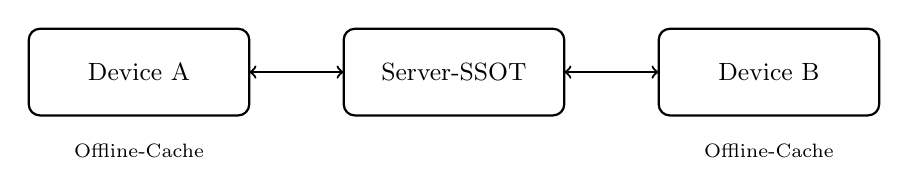
\begin{tikzpicture}[x=1cm,y=1cm]
    \draw[rounded corners, thick] (0,0) rectangle (2.8,1.1);
    \node at (1.4,0.55) {\small Device A};
    \draw[rounded corners, thick] (4,0) rectangle (6.8,1.1);
    \node at (5.4,0.55) {\small Server-SSOT};
    \draw[rounded corners, thick] (8,0) rectangle (10.8,1.1);
    \node at (9.4,0.55) {\small Device B};
    \draw[<->, thick] (2.8,0.55) -- (4,0.55);
    \draw[<->, thick] (6.8,0.55) -- (8,0.55);
    \node at (1.4,-0.45) {\scriptsize Offline-Cache};
    \node at (9.4,-0.45) {\scriptsize Offline-Cache};
  \end{tikzpicture}
  \caption{Synchronisationsmodell für Multi-Device mit zentralem Server-SSOT.}
  \label{fig:sync_model}
\end{figure}

\subsubsection{Rollen und Zugriffsrechte}
Neben Owner-Zugriffen werden in realen Szenarien rollenbasierte Rechte benötigt
(z.\,B. Nutzer, Manager, Admin). RBAC ist dafür ein etabliertes Modell, weil es
Rechte über Rollen statt über Einzelnutzer verwaltet \cite{rbacNist1996}.

\subsubsection{Datenintegrität und Validierung}
Importpfade (QR, OCR, E-Mail) erfordern mehrstufige Validierung:
\textit{syntaktisch} (Format/Pflichtfelder), \textit{semantisch}
(zeitliche Plausibilität, Betrag $>$ 0), \textit{referentiell}
(Beleg gehört zu einem gültigen Trip). Das ist auch sicherheitsrelevant, weil
unzureichende Validierung ein häufiges mobiles Risiko darstellt
\cite{owaspMobileTop10}.

\subsubsection{Konsistente Zustandstransitionen}
Wenn mehrere Tabellen fachlich zusammenhängen (z.\,B. Upload + Metadaten +
Trip-Verknüpfung), müssen Updates atomar erfolgen. ACID-Eigenschaften und
geeignete Isolationsebenen verhindern halbfertige Zustände unter Last
\cite{postgresqlTxIsolation}.

\begin{figure}[htbp]
  \centering
  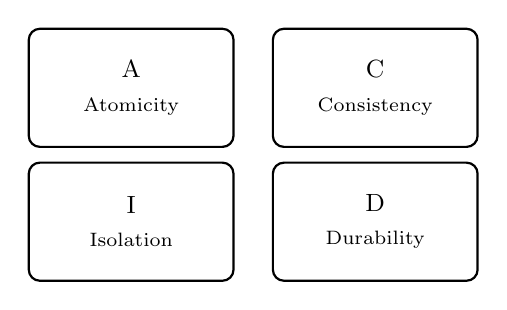
\begin{tikzpicture}[x=1cm,y=1cm]
    \draw[rounded corners, thick] (0,1.5) rectangle (2.6,3);
    \node[align=center] at (1.3,2.25) {\small A\\\scriptsize Atomicity};
    \draw[rounded corners, thick] (3.1,1.5) rectangle (5.7,3);
    \node[align=center] at (4.4,2.25) {\small C\\\scriptsize Consistency};
    \draw[rounded corners, thick] (0,-0.2) rectangle (2.6,1.3);
    \node[align=center] at (1.3,0.55) {\small I\\\scriptsize Isolation};
    \draw[rounded corners, thick] (3.1,-0.2) rectangle (5.7,1.3);
    \node[align=center] at (4.4,0.55) {\small D\\\scriptsize Durability};
  \end{tikzpicture}
  \caption{ACID als Integritätsfundament für transaktionale Updates.}
  \label{fig:acid_foundation}
\end{figure}

\subsection{Sicherheitskonzept und Datenschutz}
Ein belastbares Sicherheitsmodell kombiniert Identität, Autorisierung,
Storage-Schutz, sichere Kommunikation und Datenschutz-Governance. Als
Bedrohungsrahmen dienen mobile Top-Risiken wie unsichere Authentifizierung,
fehlende Zugriffskontrolle, unsichere Datenspeicherung und Misconfiguration
\cite{owaspMobileTop10}.

\subsubsection{Authentifizierung: Sessions, Tokens und Identität}
Token-basierte Sessions sind im Mobile-Backend Standard. JWT ist dabei ein
etabliertes Format für signierte Claims \cite{rfc7519}; OAuth 2.0 bildet den
Rahmen für delegierte Zugriffe über externe Identitätsprovider
\cite{rfc6749}. In Skyline wird dies mit Supabase Auth kombiniert, wodurch
Session-Claims und Datenbankberechtigungen zusammengeführt werden
\cite{supabaseAuth,supabaseRLS}.

\begin{figure}[htbp]
  \centering
  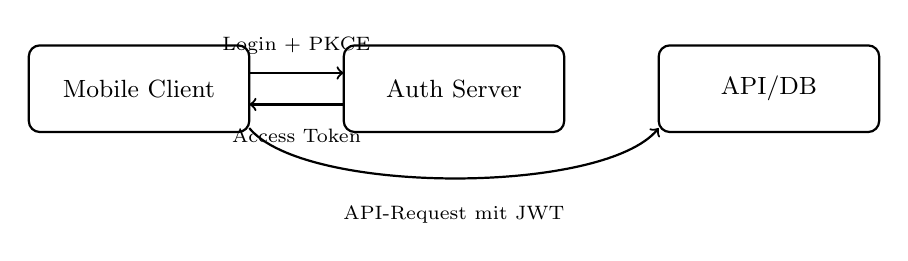
\begin{tikzpicture}[x=1cm,y=1cm]
    \draw[rounded corners, thick] (0,0) rectangle (2.8,1.1);
    \node at (1.4,0.55) {\small Mobile Client};
    \draw[rounded corners, thick] (4,0) rectangle (6.8,1.1);
    \node at (5.4,0.55) {\small Auth Server};
    \draw[rounded corners, thick] (8,0) rectangle (10.8,1.1);
    \node at (9.4,0.55) {\small API/DB};
    \draw[->, thick] (2.8,0.75) -- (4,0.75);
    \node at (3.4,1.1) {\scriptsize Login + PKCE};
    \draw[->, thick] (4,0.35) -- (2.8,0.35);
    \node at (3.4,-0.05) {\scriptsize Access Token};
    \draw[->, thick] (2.8,0.05) .. controls (3.5,-0.8) and (7.3,-0.8) .. (8,0.05);
    \node at (5.4,-1.05) {\scriptsize API-Request mit JWT};
  \end{tikzpicture}
  \caption{Vereinfachter OAuth/JWT-Flow für mobile Authentifizierung.}
  \label{fig:oauth_jwt_flow}
\end{figure}

\subsubsection{Autorisierung: Row Level Security und Policies}
Autorisierung beantwortet nicht \glqq wer bist du?\grqq{}, sondern
\glqq was darfst du sehen/ändern?\grqq{}. Row Level Security (RLS) erlaubt
Policy-getriebene Rechteprüfung auf Zeilenebene in der Datenbank
\cite{supabaseRLS}. Das folgt dem Prinzip \textit{default deny}: ohne passende
Policy kein Datenzugriff.

\subsubsection{Storage-Sicherheit für Dokumente}
Reisedokumente und Belege dürfen nicht öffentlich zugänglich sein.
Private Buckets, signierte URLs und Policy-gebundene Zugriffe bilden deshalb den
Standardansatz \cite{supabaseStorage}. Damit bleibt die Zugriffskontrolle nicht
nur in der App-Logik, sondern wird am Datenkern erzwungen.

\subsubsection{Kommunikation, Konfiguration und Logging}
Sichere Transportwege, sauberes Secret-Management und restriktive
Produktionskonfiguration sind Pflicht. Logging muss zwei Ziele gleichzeitig
erfüllen: Fehlersuche ermöglichen, aber keine sensitiven Inhalte unnötig
persistieren (z.\,B. Tokens, Volltexte von Dokumenten).

\subsubsection{DSGVO-Konsequenzen für die Architektur}
Die DSGVO wirkt unmittelbar auf technische Entscheidungen:
\begin{itemize}
  \item \textbf{Datenminimierung (Art. 5):} nur notwendige Daten speichern.
  \item \textbf{Privacy by Design/Default (Art. 25):} Zugriff standardmäßig
  restriktiv auslegen.
  \item \textbf{Löschbarkeit (Art. 17):} End-to-End-Löschpfad für Datensätze
  und Dateien vorsehen.
  \item \textbf{Sicherheit der Verarbeitung (Art. 32):} Vertraulichkeit,
  Integrität, Verfügbarkeit und Resilienz technisch absichern.
\end{itemize}
Diese Anforderungen sind für eine Reiseorganisations-App nicht optional, sondern
Teil der Kernfunktionalität \cite{gdpr}.

\section{Anforderungen an eine mobile Reiseorganisations-App}
\subsection{Durchgängiger Datenfluss}
Der fachliche Kern ist ein stabiler End-to-End-Fluss:
\textbf{Import} $\rightarrow$ \textbf{Validierung} $\rightarrow$
\textbf{Speicherung} $\rightarrow$ \textbf{Synchronisierung} $\rightarrow$
\textbf{Abfrage/Anzeige}. Dieser Fluss muss auch unter Fehlerbedingungen
(Offline, unvollständige Scans, API-Timeouts) robust degradieren können.

\begin{figure}[htbp]
  \centering
  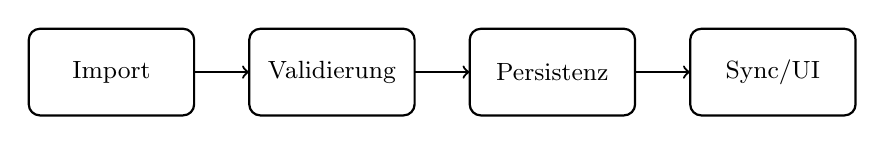
\begin{tikzpicture}[x=1cm,y=1cm]
    \draw[rounded corners, thick] (0,0) rectangle (2.1,1.1);
    \node at (1.05,0.55) {\small Import};
    \draw[rounded corners, thick] (2.8,0) rectangle (4.9,1.1);
    \node at (3.85,0.55) {\small Validierung};
    \draw[rounded corners, thick] (5.6,0) rectangle (7.7,1.1);
    \node at (6.65,0.55) {\small Persistenz};
    \draw[rounded corners, thick] (8.4,0) rectangle (10.5,1.1);
    \node at (9.45,0.55) {\small Sync/UI};
    \draw[->, thick] (2.1,0.55) -- (2.8,0.55);
    \draw[->, thick] (4.9,0.55) -- (5.6,0.55);
    \draw[->, thick] (7.7,0.55) -- (8.4,0.55);
  \end{tikzpicture}
  \caption{Kernpipeline einer mobilen Reiseorganisations-App.}
  \label{fig:core_pipeline}
\end{figure}

\subsection{Importanforderungen: QR, OCR, E-Mail}
QR-/Barcode-Import auf Basis von BCBP-Standards ist für den Flugkontext
besonders nutzerfreundlich, weil zentrale Felder strukturiert auslesbar sind
\cite{iataBCBP}. OCR und E-Mail-Import erweitern die Abdeckung, sind aber
probabilistisch und fehleranfälliger. Daraus folgt die Pflicht zu einem
\textit{human-in-the-loop}-Design: Extrahierte Felder werden als Vorschläge
angezeigt und erst nach Nutzerbestätigung als valide übernommen
\cite{mlKitTextRecognition,tesseractOcr}.

\subsection{Validierung, Zeitlogik und Speicherung}
Zeitkritische Daten (z.\,B. Boarding, Check-in-Fenster) erfordern mehr als
Formatprüfung: Zeitzonen, Datumswechsel und Plausibilität müssen
anwendungsseitig geprüft werden. Datenbankseitige Constraints und transaktionale
Speicherung bleiben das Rückgrat für konsistente Zustände
\cite{postgresqlConstraints,postgresqlTxIsolation}.

\subsection{Synchronisierung, Offline und Konflikte}
Offline-Unterstützung verbessert Nutzbarkeit unterwegs deutlich. Gleichzeitig
müssen Konflikte bei späterer Synchronisierung modelliert werden
\cite{firestoreOffline,amplifyConflict}. Für Skyline ist ein pragmatischer Ansatz
sinnvoll: konfliktarme Datenstrukturen und gezielte Konfliktlogik nur dort, wo
realistisch parallele Änderungen auftreten.

\subsection{Integrationsanforderungen}
Integrationen steigern den Nutzen, vergrößern aber die Angriffsoberfläche:
Geovisualisierung benötigt saubere Datenmodellierung; Benachrichtigungen
benötigen konsistente Zeitdaten und Privacy Controls am Sperrbildschirm
\cite{androidNotifications}.

\section{Technische Grundlagen der mobilen App-Entwicklung}
\subsection{Cross-Platform-Frontend mit React Native und Expo}
React Native ermöglicht plattformübergreifende UI- und Logikentwicklung für
iOS und Android \cite{reactNative}. Expo vereinfacht Build-, Deployment- und
Update-Prozesse durch ein integriertes Tooling-Oekosystem
\cite{expoDocs,easBuild,easUpdate}.

\subsection{Backend-as-a-Service mit Datenbank- und Security-Nähe}
Supabase kombiniert Postgres, Auth, Storage und Realtime in einer integrierten
Plattform \cite{supabasePlatform}. Für diese Arbeit ist besonders relevant, dass
RLS und Storage-Policies direkt an der Datenebene greifen
\cite{supabaseRLS,supabaseStorage,supabaseAuth}.

\subsection{Technologievergleich und Architekturentscheidung}
Für eine Reiseorganisations-App sind insbesondere vier Vergleichskriterien
tragfähig: Datenintegrität, Rechteverwaltung, Offline-Verhalten und
Compliance-Fähigkeit.

\begin{table}[htbp]
  \centering
  \caption{Vergleich möglicher Architekturpfade für mobile Reiseorganisation}
  \label{tab:architekturvergleich}
  \begin{tabular}{p{3.1cm}p{4.1cm}p{5.8cm}}
    \textbf{Pfad} & \textbf{Stärken} & \textbf{Trade-offs} \\
    \midrule
    Postgres-zentrierte BaaS (RLS) &
    starke Integrität, klare Relationen, Policy-Logik am Datenkern &
    Offline-Konzept muss bewusst modelliert werden \\
    \midrule
    NoSQL-Realtime mit Offline-Persistenz &
    schnelle Sync-UX, Realtime by default &
    relationale Konsistenzregeln häufig anwendungsseitig \\
    \midrule
    Offline-first Sync-Framework &
    explizite Konfliktstrategien, gute Multi-Device-Unterstützung &
    höhere Plattformkomplexität und Resolver-Aufwand \\
  \end{tabular}
\end{table}

Für Skyline überwiegt ein relationales Zentrum mit RLS, weil Datenintegrität,
Nachvollziehbarkeit und zugriffsbasierte Sicherheit im Projektkontext priorisiert
sind. Offline-Fähigkeit wird ergänzend über lokale Datenhaltung und
kontrollierte Synchronisierung umgesetzt.
